\documentclass{article}

% Packages for formatting and special symbols
\usepackage{amsmath}
\usepackage{amssymb}
\usepackage{graphicx}
\usepackage{caption}
\usepackage{subcaption}
\usepackage{hyperref}
\usepackage{geometry}
\usepackage{fancyhdr}
\usepackage{setspace}
\usepackage{enumitem}
\usepackage{float}

\graphicspath{ {./graphs/} }

% Page layout
\geometry{top=1in, bottom=1in, left=1in, right=1in} % Adjust margins as needed
\pagestyle{fancy}
\fancyhf{}
\rhead{Matic Stare}
\lhead{Izločanje očesnih artefaktov z uporabo postopka analize neodvisnih komponent (ANK)}
\cfoot{\thepage}
\renewcommand{\headrulewidth}{0.4pt}
\renewcommand{\footrulewidth}{0.4pt}
\begin{document}
% Title
\title{Izločanje očesnih artefaktov z uporabo postopka analize neodvisnih komponent (ANK)}
\author{Matic Stare}
\date{\today}



\maketitle

% Sections
\section{Uvod}
\label{sec:introduction}

Preden začnemo z obravnavo EEG signalov je potrebno odstraniti očesne artefakte, na katere vpliva gibanje oči. V tem članku bomo predstavili postopek analize neodvisnih komponent (ANK), ki je namenjen odstranjevanju očesnih artefaktov iz EEG signalov. Implementirali smo program, ki s pomočjo algoritma FastICA izvede dekompozicijo EEG signala na neodvisne komponente.


\section{Metode}
\label{sec:methodology}

Iz podatkovne baze EEGMMI (ki je dostopna na povezavi \href[]{https://www.physionet.org/content/eegmmidb/1.0.0/}{Physionet}) smo naključno izbrali en subjekt. Ker poskušamo izločiti očesne artefakte, smo izbrali prvo vajo, pri kateri je imel subjekt odprte oči. Program smo implementirali v programskem okolju MATLAB. Za branje EEG signalov, pa smo si pomagali s paketom WFDB. Za izvedbo ANK smo uporabili algoritem FastICA, ki smo ga uporabili tudi na laboratorijskih vajah. Z namenom, da bi vse komponente konvergirale, smo nastavili maksimalno število iteracij na 5000. Program smo testirali na posnetku \textbf{S020R01.edf}.

\section{Rezultati}
\label{sec:results}
Na sliki \ref{fig:decomposed} pa so prikazani signali posameznih elektrod. Vidimo lahko, da se komponente med 22 in 38 precej razlikujejo od ostalih. To ni naklučje, saj so to ravno komponente elektrod, ki so pritrjene blizu oči.

Na sliki \ref{fig:original} je prikazan originalni EEG signal. Na sliki \ref{fig:newSigs} so prikazani signali, ki smo jih dobili po odstranitvi komponent, ki so povezane z očesnimi artefakti. Vidimo lahko, da signali nimajo več toliko odstopanj, kot so jih imeli v originalnem signalu.


\begin{figure}[H]
    \centering
    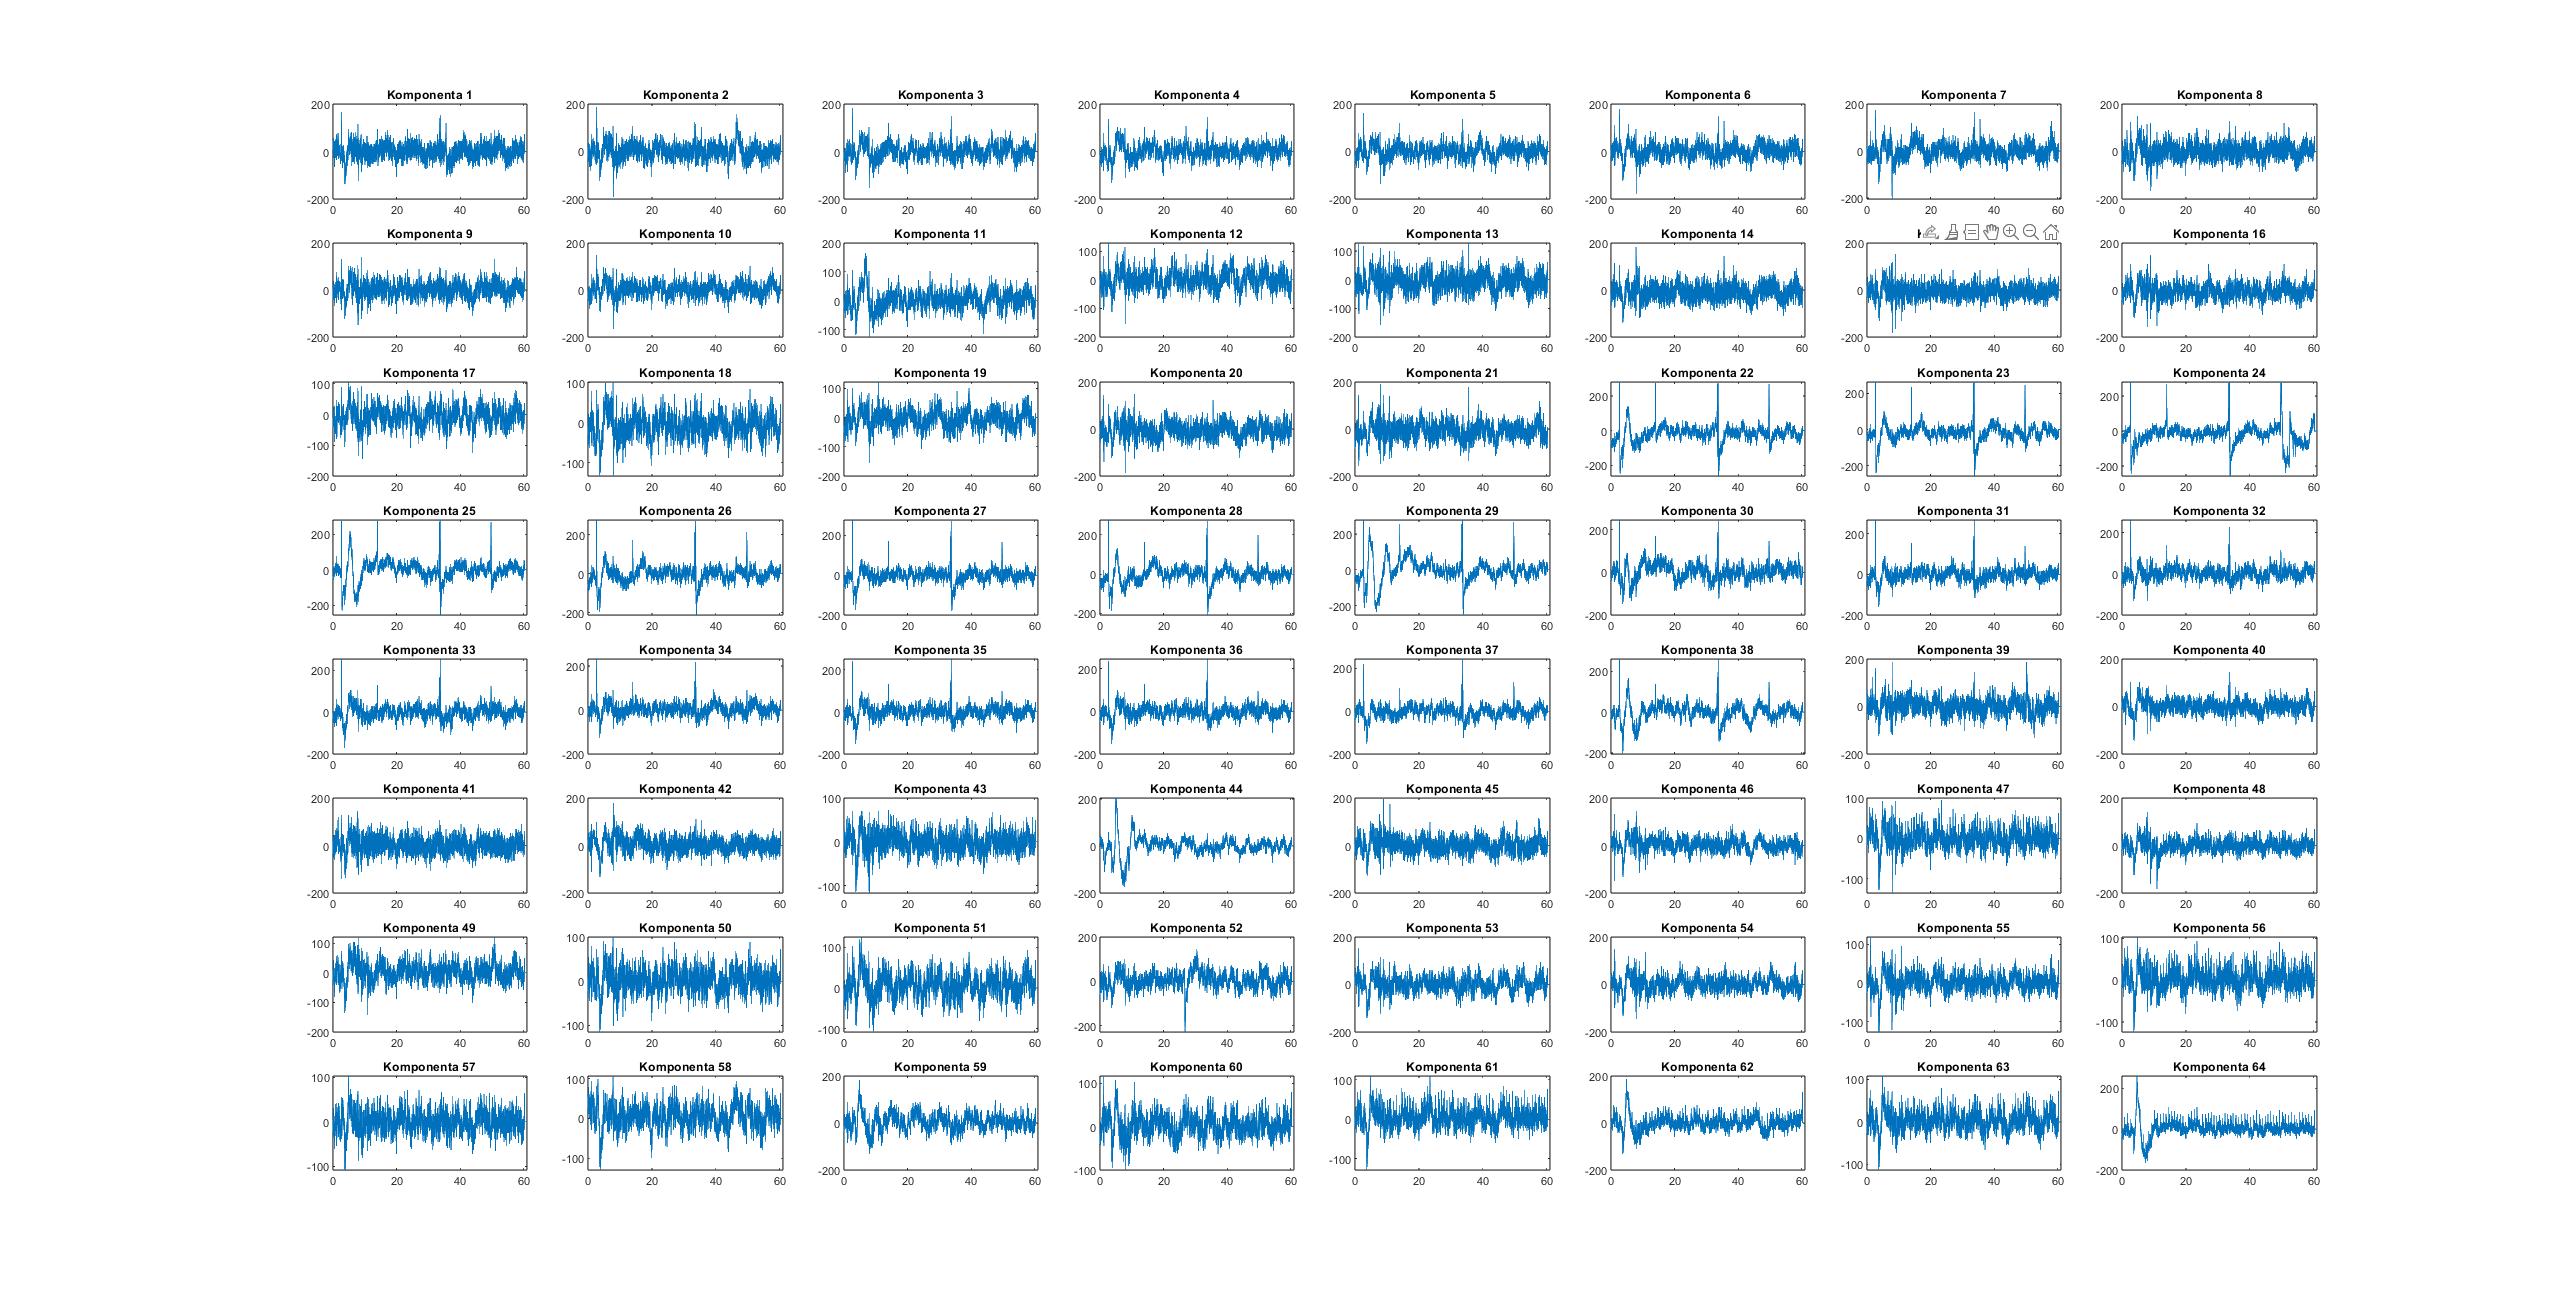
\includegraphics[width=\textwidth]{decompSigs.png}
    \caption{Signali posameznih elektrod.}
    \label{fig:decomposed}
\end{figure}



\begin{figure}[H]
    \begin{subfigure}{0.49\linewidth}
        \centering
        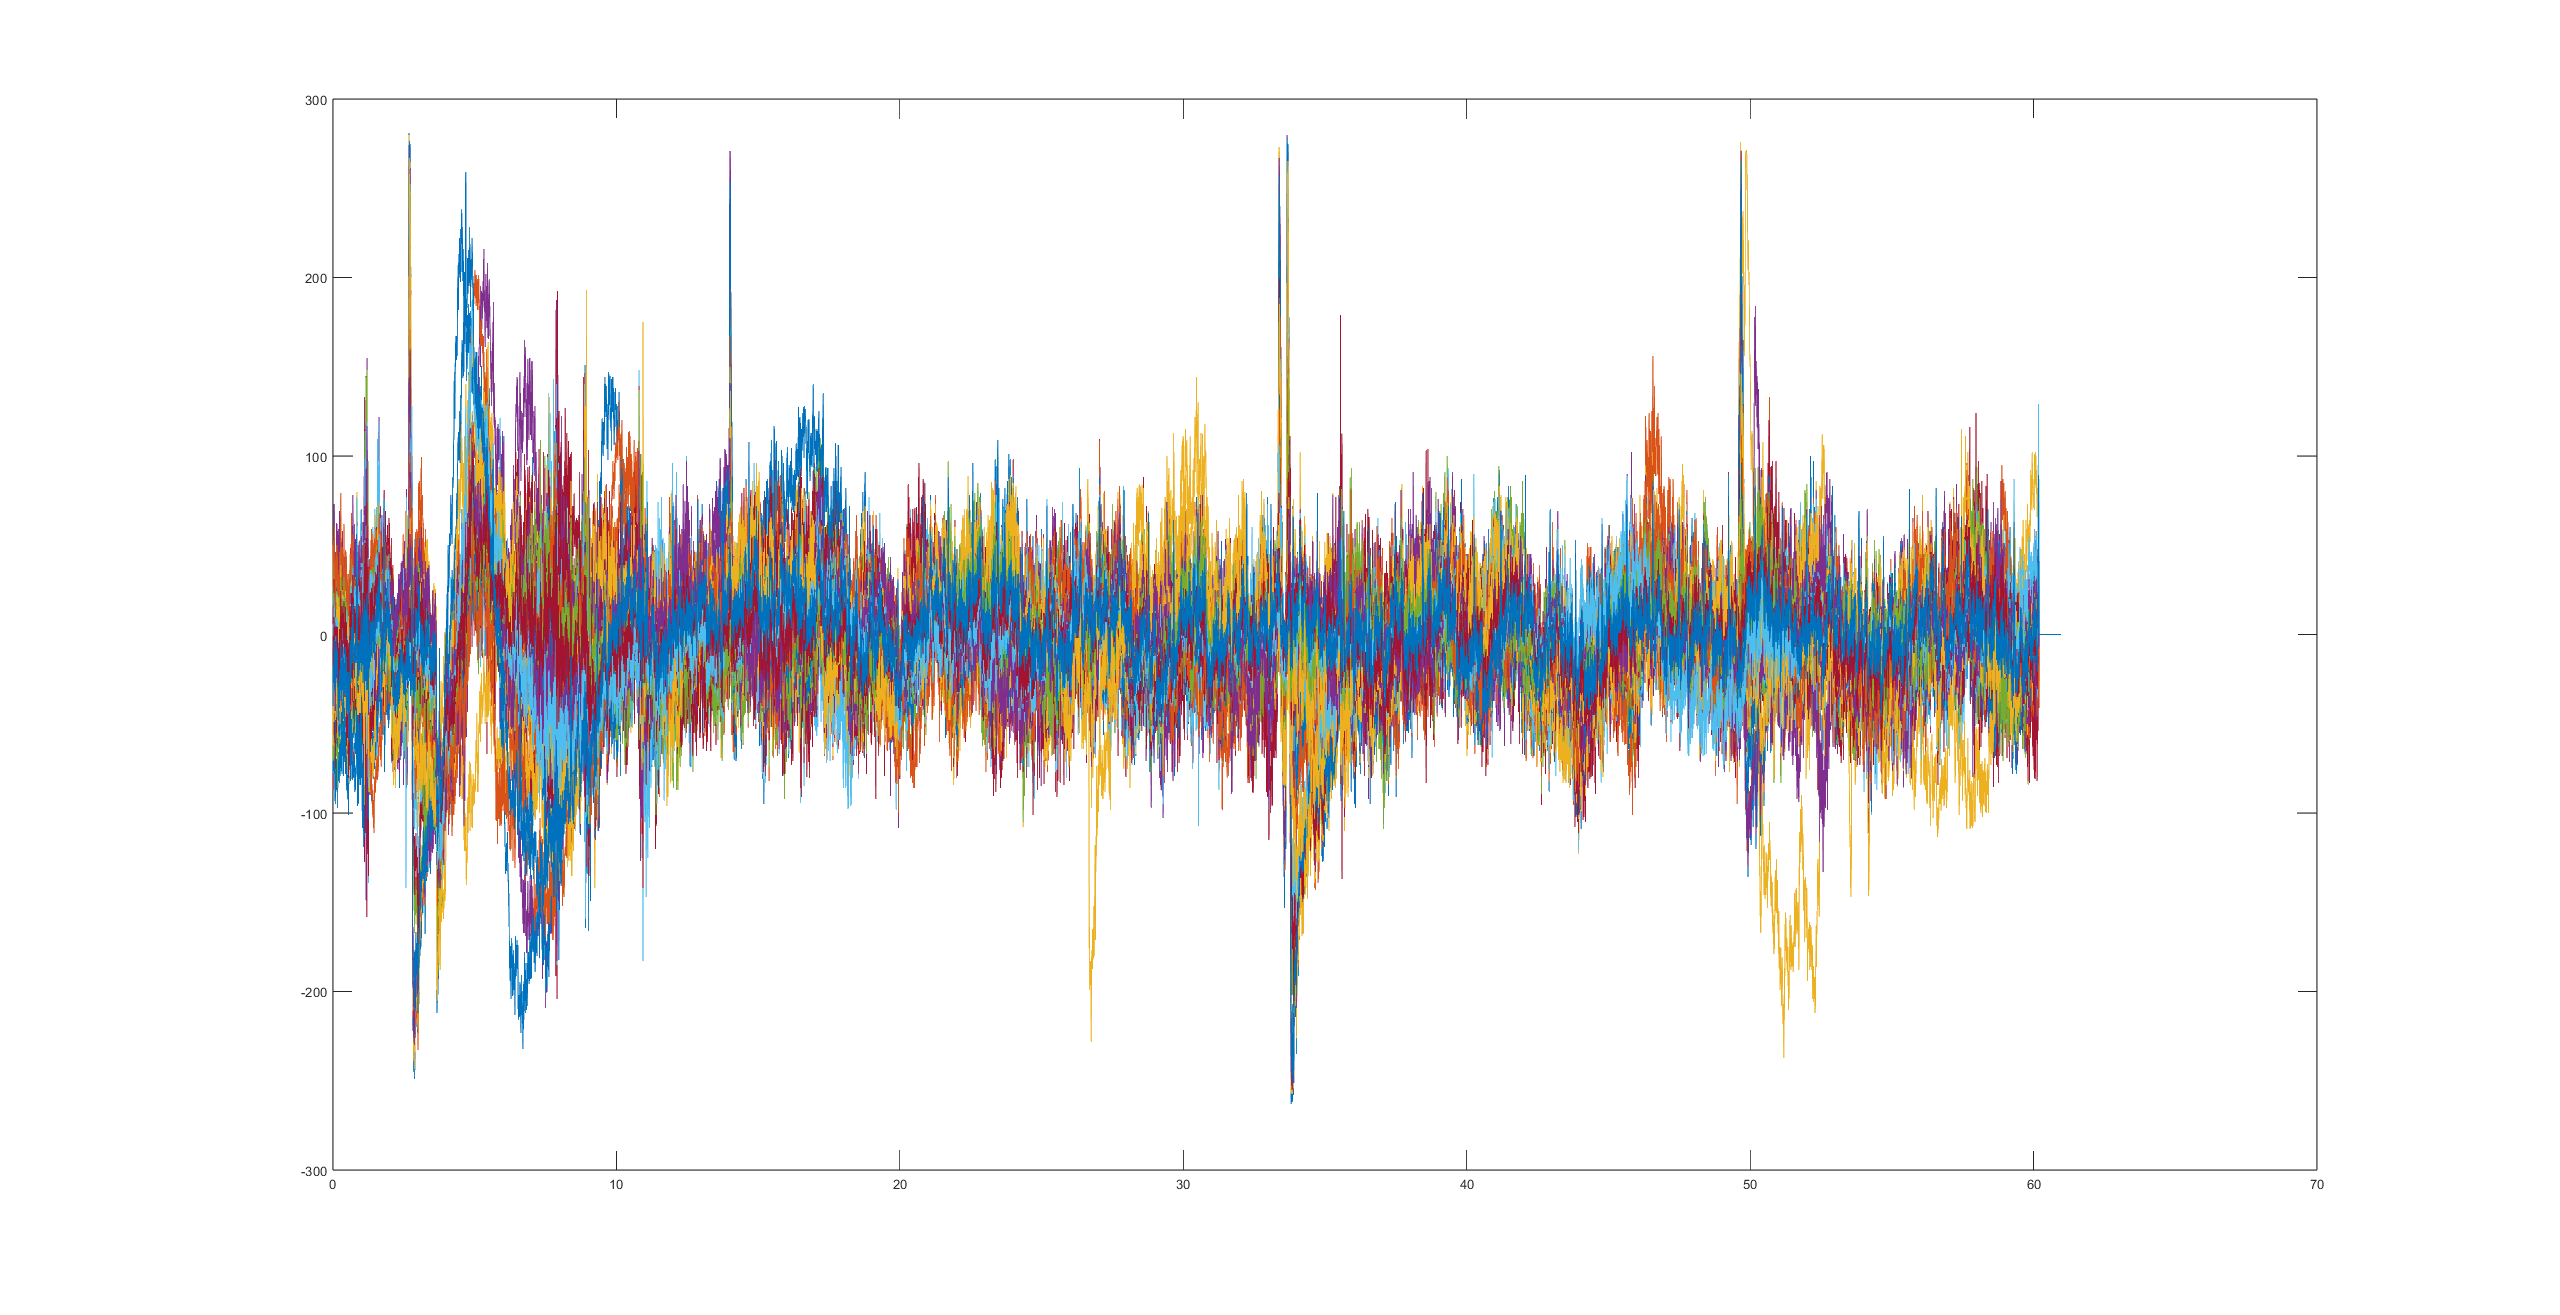
\includegraphics[width=\textwidth]{sigs.png}
        \caption{Originalni EEG signal.}\label{fig:original}
    \end{subfigure}
    \begin{subfigure}{0.49\linewidth}
        \centering
        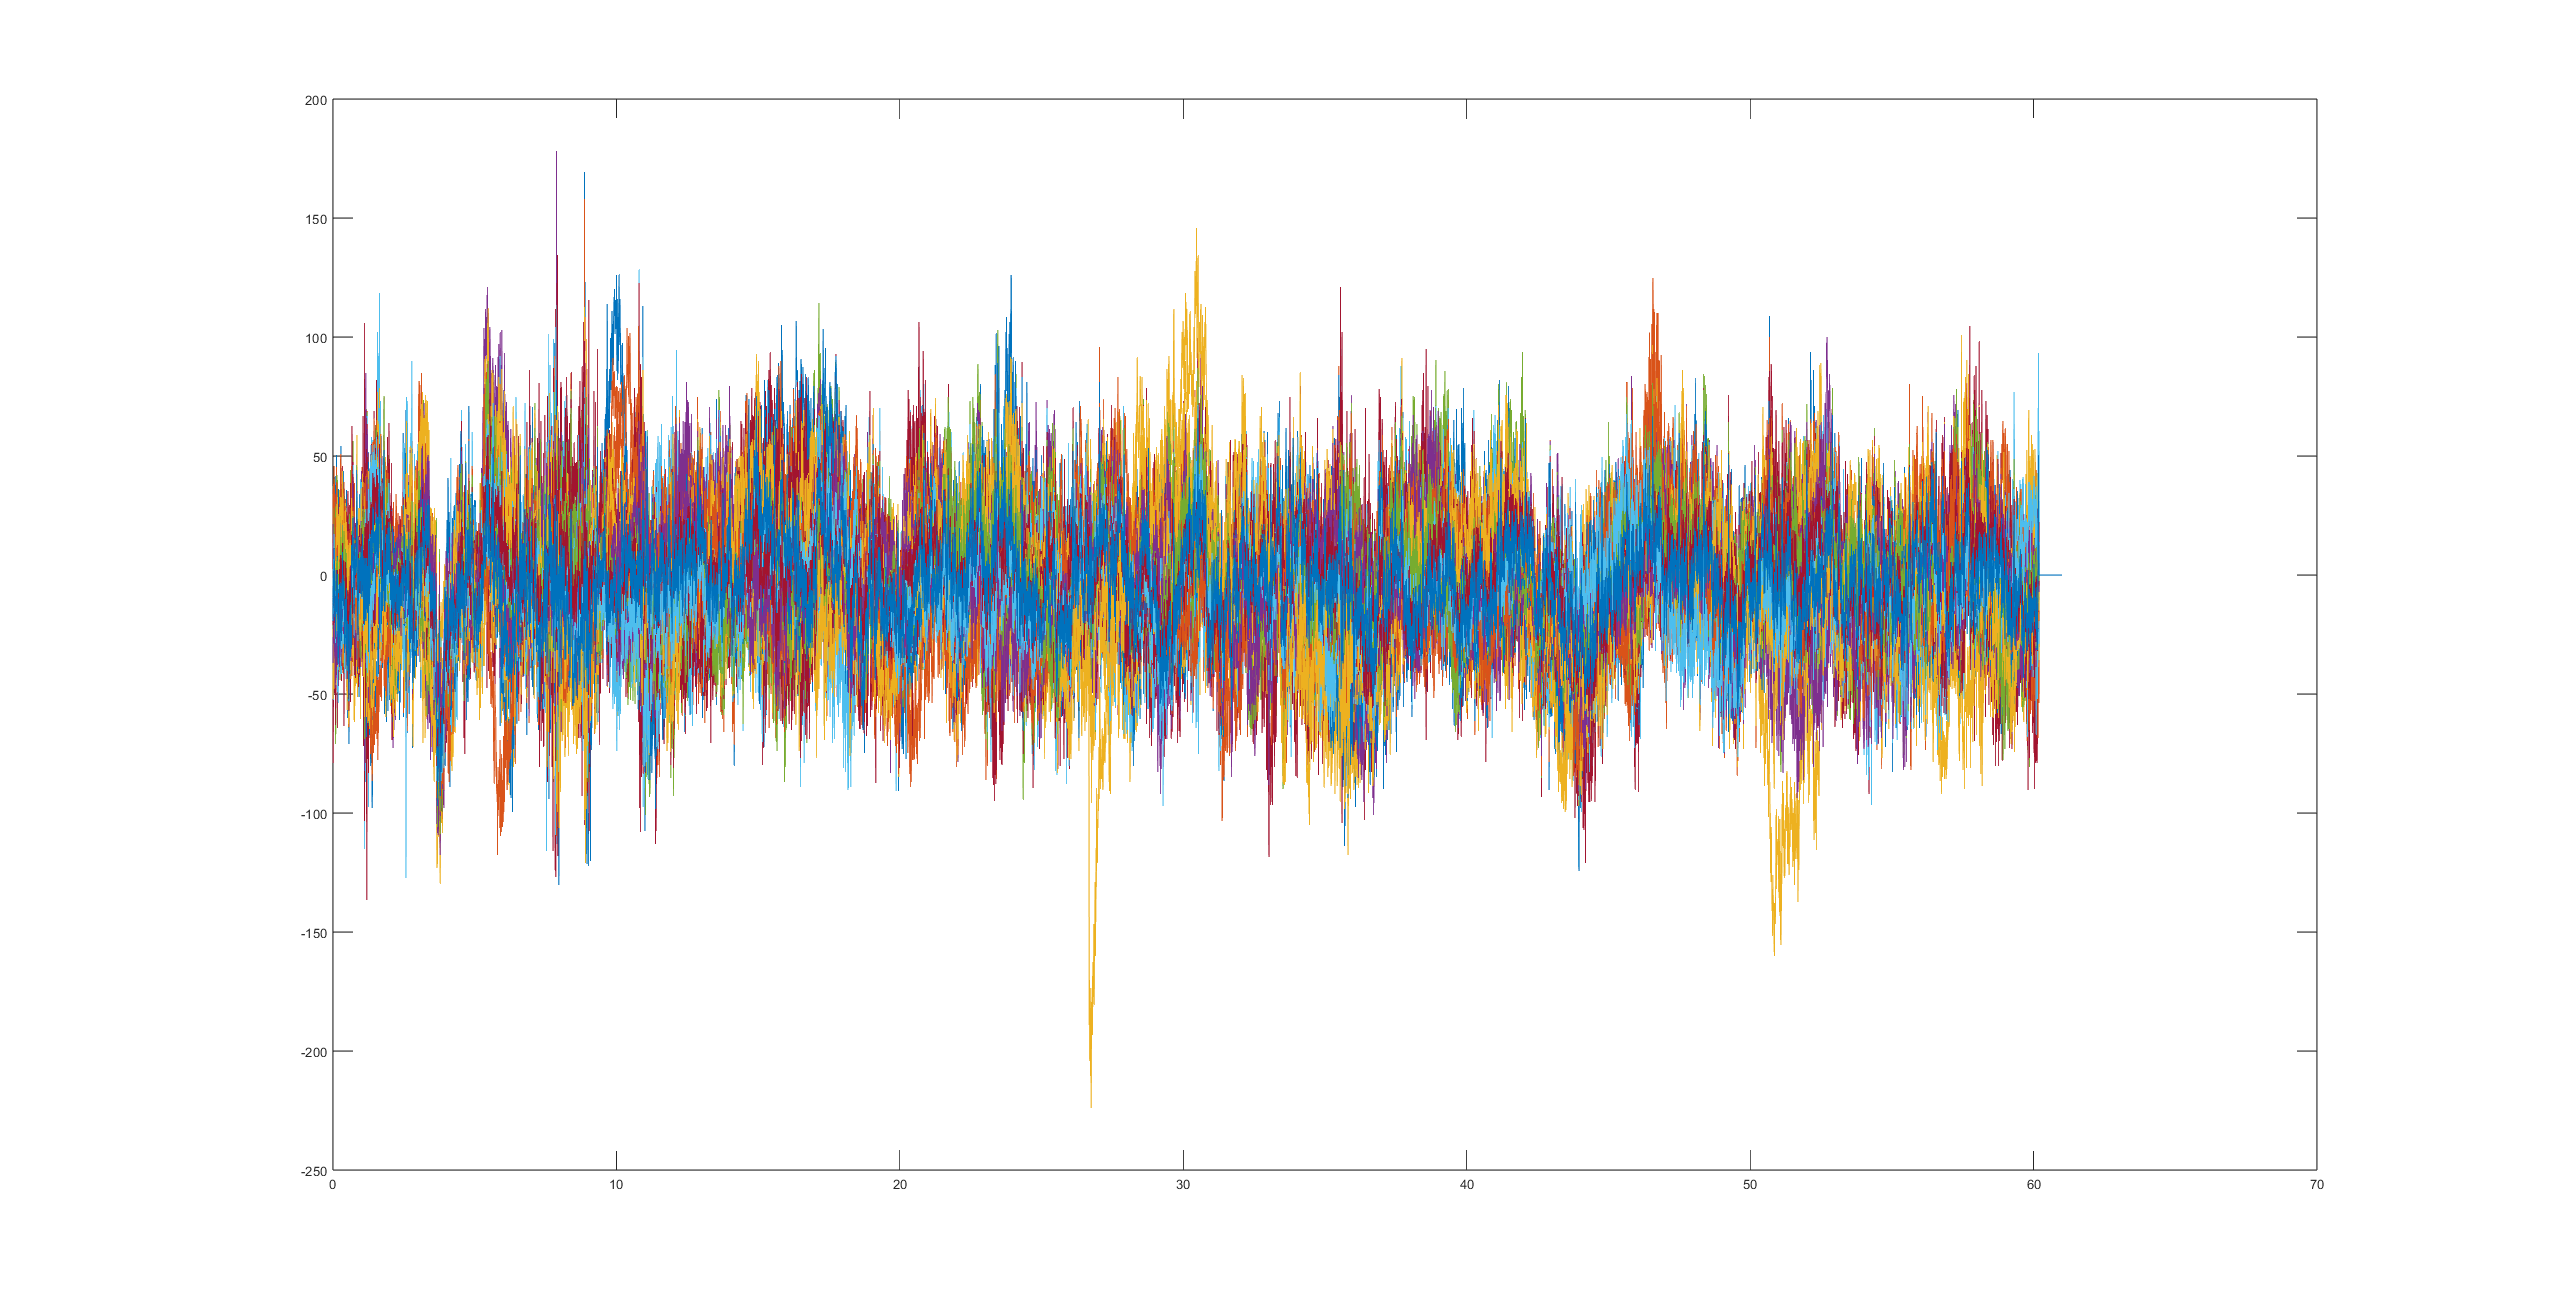
\includegraphics[width=\textwidth]{newSigs.png}
        \caption{EEG signal z odstranjenimi očesnimi artefakti.}\label{fig:newSigs}
    \end{subfigure}
    \caption{Before and after graph}\label{fig:beforeAfter}
\end{figure}


\section{Diskusija}
\label{sec:discussion}

Vidimo lahko, da je postopek ANK zelo učinkovit pri odstranjevanju očesnih artefaktov, saj je v novem signalu precej manj šuma. Vendar pa je potrebno biti previden pri izbiri komponent, ki jih želimo odstraniti. V našem primeru smo odstranili komponente, ki so bile povezane z očesnimi artefakti. Kot nadalnje delo, bi lahko poskusili odstraniti tudi komponente, ki so povezane z drugimi artefakti.

\end{document}